% =====================================================================================================
\section{Hardware Architecture}\label{sec:hardware}
\begin{figure*}[t]
\centering
\resizebox{\textwidth}{!}{% Fabric datapath of the contract-v3 lane encoder (rtl/secure_jpeg_lanes_top.v, rtl/encoder_lane.v).
% Bus widths are the RTL port widths; module names are the RTL file names.
\begin{tikzpicture}[x=1cm, y=1cm, st/.style={pl, minimum height=9mm, minimum width=13.5mm, font=\tiny}]
% ---- input and dealer
\node[blk, fill=netfill, font=\tiny, minimum height=9mm] (in) at (0,0) {s\_axis\\64\,b\\2 px/beat};
\node[pl, font=\tiny, minimum height=24mm, minimum width=11mm, align=center] (deal) at (1.45,-0.75) {dealer\\[2pt]MCU row\\$r\to$ lane\\$r \bmod L$};
\draw[bus] (in) -- (in -| deal.west);
% ---- lane 0 (full) -- y = 0
\node[st] (cc0)  at (3.05,0) {rgb2ycbcr\\2px $\to$ 1\\sample/clk};
\node[st] (dct0) at (4.65,0) {dct8x8\\two-pass\\13-bit};
\node[st] (q0)   at (6.25,0) {quantiser\\$\times R_{uv}$,\\$\gg 16$};
\node[st] (zz0)  at (7.85,0) {zigzag\_rle\\DC pred.\\reset/seg.};
\node[st, fill=cryfill] (se0) at (9.45,0) {selective\\\_enc\\(XOR)};
\node[st] (hu0)  at (11.05,0) {huffman\\\_enc\\(Annex K)};
\node[st] (bp0)  at (12.65,0) {bit\_packer\\stuff, pad\\per seg.};
\node[st, minimum width=10mm] (ff0)  at (14.05,0) {byte\\FIFO\\2\,KB};
\node[cry, font=\tiny, minimum width=19mm, minimum height=8mm] (ks0) at (9.45,1.25) {keystream\_gen\\Ascon$(K_{\mathrm{seg}}, N_{s,t})$};
\draw[arr] (ks0) -- node[lbl, left, align=right]{16-bit window,\\take $n\le 12$ bits} (se0);
\draw[arr] (deal.east |- cc0) -- (cc0);
\draw[arr] (cc0) -- node[lbl, above]{8} (dct0);
\draw[arr] (dct0) -- node[lbl, above]{16} (q0);
\draw[arr] (q0) -- node[lbl, above]{16} (zz0);
\draw[arr] (zz0) -- node[lbl, above]{20} (se0);
\draw[arr] (se0) -- node[lbl, above]{20} (hu0);
\draw[arr] (hu0) -- node[lbl, above]{32} (bp0);
\draw[arr] (bp0) -- node[lbl, above]{8} (ff0);
\begin{scope}[on background layer]
\node[grp, fill=plfill!30, fit=(cc0)(ff0)(ks0), inner sep=1.6mm, label={[font=\tiny\bfseries, anchor=south west, inner sep=1pt]north west:encoder\_lane 0}] (lane0) {};
\end{scope}
% ---- lane L-1 (collapsed) -- y = -1.6
\node[pl, font=\tiny, text width=118mm, minimum height=7mm, align=center] (laneL) at (8.46,-1.8) {the same pipeline (colour, DCT, quantiser, zig-zag + RLE, \textbf{selective XOR}, Huffman, packer, FIFO) with its own keystream generator};
\node[font=\tiny\bfseries, anchor=south west] at (laneL.north west) {encoder\_lane $L{-}1$ \ (lanes $1 \ldots L{-}1$; $L = 1, 2, 4$)};
\draw[arr] (deal.east |- laneL) -- (laneL);
% ---- merger, tag, word packer
\node[pl, font=\tiny, minimum height=24mm, minimum width=13mm, align=center] (mrg) at (16.0,-0.75) {segment\\\_merger\\[2pt]seg.\ $s$ from\\lane $s \bmod L$\\(E5: $\lfloor s/c\rfloor$\\$\bmod L$)\\[2pt]+ RST$_{s \bmod 8}$};
\draw[arr] (ff0.east) -- (ff0.east -| mrg.west);
\draw[arr] (laneL.east) -- (laneL.east -| mrg.west);
\node[cry, font=\tiny, minimum width=18mm, minimum height=9mm] (tag) at (18.15,0.35) {tag\_unit\\Ascon MAC over\\prefix $\|$ scan};
\node[pl, font=\tiny, minimum width=18mm, minimum height=9mm] (wp) at (18.15,-1.85) {scan\_word\\\_packer\\32\,b + TKEEP};
\draw[arr] (mrg.east |- tag) -- node[lbl, above]{8} (tag.west);
\draw[arr] (mrg.east |- wp) -- node[lbl, above]{8} (wp.west);
\node[blk, fill=netfill, font=\tiny, minimum height=8mm] (out) at (18.15,-3.1) {m\_axis 32\,b};
\draw[bus] (wp) -- (out);
% ---- per-frame key, registers
\node[cry, font=\tiny, minimum width=24mm, minimum height=8mm] (kseg) at (5.6,2.85) {kseg\_unit: $K_{\mathrm{seg}}$ =\\Ascon-MAC$(K, N^{\mathrm{enc}}_t, \text{``lanes''})$};
\draw[arr] (kseg.east) -| node[lbl, pos=0.75, right]{$K_{\mathrm{seg}}$, once per frame, to every lane} (ks0.north);
\node[pl, font=\tiny, minimum width=24mm, minimum height=8mm] (regs) at (1.6,2.85) {axil\_regs\\$K$, $\sigma$, $t$, mode, size, $R_{uv}$};
\draw[arr] (regs) -- (kseg);
\draw[arr] (regs.north) -- ++(0,0.3) -| node[lbl, pos=0.25, above]{$K$ and the 26-byte prefix (mode, $\sigma$, $t$, $W$, $H$)} (tag.north);
\draw[arr] (tag.south) ++(0.5,0) -- ++(0,-0.35) node[lbl, right]{$T$ to TAG0--3};
\end{tikzpicture}
}
\caption{Fabric datapath of the lane encoder \texttt{secure\_jpeg\_lanes\_top} (module names are the RTL files; numbers on arrows are bus widths in bits). The dealer sends MCU row $r$ to lane $r \bmod L$; each lane converts, transforms, quantizes and entropy-codes its restart segments with its own keystream; the merger restores raster order and inserts restart markers; the tag unit authenticates the prefix and the merged scan. The single-pipeline encoder is one lane without dealer and merger.}
\label{fig:pl}
\end{figure*}
\subsection{Datapath}\label{sec:datapath}
Fig.~\ref{fig:pl} shows the encoder. All stages are joined by valid/ready handshakes and tolerate back-pressure from the DMA, which the testbenches check with random stalls. The colour converter takes two pixels per clock into block-RAM line buffers, the DCT is two passes of an eight-tap multiply-accumulate, the quantizer multiplies by a reciprocal table in one DSP slice, and the zig-zag stage emits one symbol per clock and resets its DC predictors at every segment, ahead of encryption, Huffman coding and byte packing. The merger copies the segments of all lanes in raster order and writes the restart markers, and the tag unit absorbs the prefix and every merged byte into an Ascon core.

\subsection{Circuit of the encryption stage}\label{sec:circuit}
\begin{figure}[t]
\centering
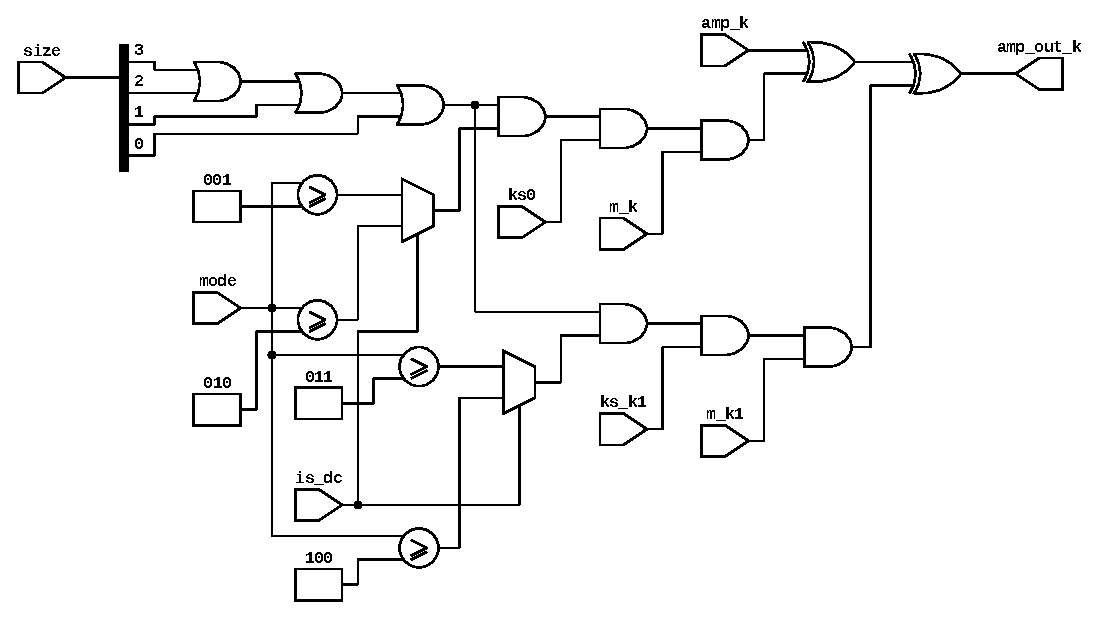
\includegraphics[width=\columnwidth]{figures/fig_selective_enc_bitslice.pdf}
\caption{Gate-level circuit of bit slice $k$ of \texttt{selective\_enc.v}, generated from the RTL by Yosys and netlistsvg: comparators on the mode and multiplexers selected by is\_dc form the sign and amplitude enables; two XORs implement~\eqref{eq:slice}. $m_k = [k < s]$; ks0 and ks\_k1 are keystream bits 0 and $k{+}1$. A test simulates the slice exhaustively against the golden model.}
\label{fig:circuit}
\end{figure}
Fig.~\ref{fig:circuit} is one bit slice of the stage. The control part decodes $\gamma = [s \ne 0] \wedge (\text{is\_dc} \mathbin{?} \text{mode} \ge 2 : \text{mode} \ge 1)$ and $\alpha = [s \ne 0] \wedge (\text{is\_dc} \mathbin{?} \text{mode} \ge 4 : \text{mode} \ge 3)$; mode 5 selects the fields of mode 4 because all comparisons are $\ge$. The data part is eleven identical slices,
\begin{equation}
\amp'_k = \amp_k \xor (\gamma z_0 \wedge m_k) \xor (\alpha z_{k+1} \wedge m_{k+1}), \quad m = 2^s - 1,
\label{eq:slice}
\end{equation}
one XOR deep after the masks, which are computed one register earlier. The stage accepts a symbol when its output is free and at least $n$ keystream bits are available.

\textit{Keystream window.} \texttt{keystream\_gen} holds two 128-bit blocks and a pointer to the next unused bit and presents a 16-bit window; taking $n$ bits advances the pointer, and a new block is requested whenever fewer than two are held or in flight.

\begin{proposition}[The cipher never stalls the encoder]\label{prop:supply}
Once the first keystream block of a segment is available, the encryption stage never waits for keystream bits.
\end{proposition}
\begin{IEEEproof}
The stage accepts at most one symbol per clock and takes at most 11 bits per symbol. The core produces 128 bits per data block in nine cycles (one to absorb, eight rounds), more than 14 bits per cycle, and keeps up to 256 bits buffered, more than the 16 that the window exposes. Supply exceeds the worst-case demand, so the window, once filled, never drops below what a symbol needs.
\end{IEEEproof}
The first block of a segment costs an initialization and one data block, 21 cycles, which overlaps with the previous segment; RTL simulation confirms that the cycle counts of E0--E4 differ by at most \MaxExtraCycles{} cycles per frame.

\textit{Ascon core.} \texttt{ascon\_aead128\_core} computes one round per clock: a 320-bit state register, a 4-bit round counter whose complement and value form the round constant, and the combinational round. One bit slice of the S-box layer has eleven XOR, five AND and six NOT gates, so the layer has $64 \times 22 = 1408$ gates; the linear layer adds $2 \times 320$ two-input XORs, and its rotations are wiring. The design instantiates one core per lane for keystreams, one for the segment key and one for the tag.

\subsection{Parallel lanes}\label{sec:lanes}
One pipeline consumes one sample per clock, i.e.\ at least 1.5 cycles per pixel. Restart segments are independent (DC predictors reset, byte alignment, own keystream), so $L$ pipelines can code segments simultaneously: the dealer sends MCU row $r$ to lane $r \bmod L$ and the merger reads segment $h$ from its lane (under E5 from lane $\lfloor h/c \rfloor \bmod L$ with $c = W/16$, tracked by counters). With a 64-bit input carrying two pixels per clock,
\begin{equation}
c_L \ge \max\Bigl(\frac{1.5}{L}, \frac{1}{2}\Bigr), \qquad \Theta_L = \frac{f_{\mathrm{clk}}}{c_L},
\label{eq:lanes}
\end{equation}
i.e.\ at most \BoundOneMpix, \BoundTwoMpix{} and \BoundFourMpix\,Mpixel/s at 100\,MHz for $L = 1, 2, 4$. The bytes do not depend on $L$. A lane encoder can also be built for a camera's YUYV (4:2:2) input: four pixels per beat, no colour multipliers, a bound of $\max(1.5/L, 1/4)$ and half the bytes read from DDR.

\subsection{System and timing closure}\label{sec:zynq}
A script builds the PYNQ-Z2 system in Vivado: the Zynq processing system, an AXI DMA on the 64-bit high-performance port and the encoder as a module reference, all on one clock (100\,MHz, or 125\,MHz for four lanes). The register map holds the key, session identifier, counter, size, mode, tag, output length and three cycle counters (start to done, waiting for pixels, waiting for the output DMA), so the board reports the fabric's own time. Timing closure needed four changes, each accepted only when every RTL test still matched the model bit for bit: a five-stage pipeline for the DCT row sums (the first implementation reached only about 47\,MHz after routing), registered pixel conversion in the complete system, a zig-zag stage split into two handshaked stages, and two-entry register slices that cut the ready chain from the packer back to the keystream pointer.
